% Shared standalone design for the editable figure reconstructions.
\documentclass[tikz,border=5pt,10pt]{standalone}
\usepackage[T1]{fontenc}
\usepackage[utf8]{inputenc}
\usepackage{newpxtext,newpxmath}
\usepackage[scaled=.94]{sourcesanspro}
\usepackage{pgfplots}
\pgfplotsset{compat=1.18}
\usetikzlibrary{arrows.meta,calc,positioning,decorations.pathreplacing,
  decorations.markings,patterns,matrix,shapes.geometric,fit,backgrounds,
  intersections,angles,quotes}
\definecolor{ink}{HTML}{203746}
\definecolor{accent}{HTML}{146C78}
\definecolor{muted}{HTML}{667780}
\definecolor{signalred}{HTML}{B94B44}
\color{ink}
\tikzset{>=Latex,line width=.8pt,
  every node/.style={font=\small},
  axis/.style={->,draw=muted,line width=.5pt},
  guide/.style={draw=muted,dashed,line width=.45pt},
  curve/.style={draw=accent,line width=1pt},
  marker/.style={circle,fill=accent,inner sep=1.5pt},
  labelbox/.style={fill=white,inner sep=2pt}}

\begin{document}
\begin{tikzpicture}
\begin{axis}[width=10.9cm,height=6.2cm,xmin=0,xmax=1.1,ymin=0,ymax=2.35,axis lines=left,xlabel={$\tau$},ylabel={$h(\tau)$},xtick={.333333,.5,.666667,1},xticklabels={$1/L$,$\frac{2}{L+\mu}$,$2/L$,$1/\mu$},ytick={.5,1},yticklabels={$\rho^\star$,$1$},tick label style={font=\footnotesize},legend style={at={(.02,.98)},anchor=north west,draw=none,fill=white,font=\small},legend cell align=left,clip=false]
\addplot[signalred,dashed,domain=0:1.1,samples=101] {abs(1-3*x)};\addlegendentry{$|1-\tau L|$}
\addplot[muted,dashed,domain=0:1.1,samples=101] {abs(1-x)};\addlegendentry{$|1-\tau\mu|$}
\addplot[accent,very thick] coordinates {(0,1) (.5,.5) (1.1,2.3)};\addlegendentry{$h(\tau)=\max(|1-\tau L|,|1-\tau\mu|)$}
\addplot[muted,dotted,forget plot] coordinates {(0,1) (1.1,1)};
\addplot[muted,dotted,forget plot] coordinates {(.5,0) (.5,.5) (0,.5)};
\addplot[only marks,accent,mark=*,mark size=2pt,forget plot] coordinates {(.5,.5)};
\node[anchor=west,fill=white,font=\small] at (axis cs:.59,.35) {$\rho^\star=\dfrac{L-\mu}{L+\mu}$};
\end{axis}
\end{tikzpicture}
\end{document}
